\documentclass[conference]{IEEEtran}
\IEEEoverridecommandlockouts
\usepackage{cite}
\usepackage{amsmath,amssymb,amsfonts,mathtools}
\usepackage{graphicx}
\usepackage{textcomp}
\usepackage{xcolor}
\usepackage{booktabs}
\usepackage{siunitx}
\usepackage{tikz}
\usetikzlibrary{arrows.meta,positioning,calc,fit}
\sisetup{detect-weight=true,mode=text}
% ======================================================================
% numbers.tex -- every number quoted in the paper that is produced by a work
% package. Update here only. Sections marked [03] / [04] are under revision.
% ======================================================================
\providecommand{\TODO}[1]{\textbf{\textcolor{red}{[TODO: #1]}}}
% ---------------- [01] system identification --------------------------
\newcommand{\Tsamp}{0.02}
\newcommand{\vTauV}{0.217}      % tau_v [s]
\newcommand{\vPoleV}{0.9119}    % pole of Gv
\newcommand{\vAone}{-0.9119}    \newcommand{\vBone}{0.0882}
\newcommand{\vGdc}{1.001}
\newcommand{\latAone}{-1.3122}  \newcommand{\latAtwo}{0.4813} \newcommand{\latBone}{0.2923}
\newcommand{\latKdelta}{1.728}  \newcommand{\latWn}{24.7} \newcommand{\latZeta}{0.74}
\newcommand{\latPoleRe}{0.6561} \newcommand{\latPoleIm}{0.2255}
\newcommand{\Kus}{0.055}        \newcommand{\csat}{1.50}
\newcommand{\fitLonIdOSA}{96.61}  \newcommand{\rLonIdOSA}{0.9989}
\newcommand{\fitLonIdFree}{92.52} \newcommand{\rLonIdFree}{0.9944}
\newcommand{\fitLonVaOSA}{97.31}  \newcommand{\rLonVaOSA}{0.9993}
\newcommand{\fitLonVaFree}{93.14} \newcommand{\rLonVaFree}{0.9953}
\newcommand{\fitLatIdOSA}{96.85}  \newcommand{\rLatIdOSA}{0.9990}
\newcommand{\fitLatIdFree}{91.94} \newcommand{\rLatIdFree}{0.9935}
\newcommand{\fitLatVaOSA}{96.95}  \newcommand{\rLatVaOSA}{0.9991}
\newcommand{\fitLatVaFree}{91.66} \newcommand{\rLatVaFree}{0.9930}
\newcommand{\fitLonChrono}{84.3}  \newcommand{\fitLatChrono}{91.6}
\newcommand{\fitLonSwap}{91.5}    \newcommand{\fitLatSwap}{91.7}
\newcommand{\fitLatBase}{85.6}    \newcommand{\fitLatSpeed}{90.4}
\newcommand{\tfssErr}{10^{-15}}
% ---------------- [02] PID --------------------------------------------
\newcommand{\lonKp}{6.820} \newcommand{\lonKi}{9.738} \newcommand{\lonKd}{0.9396} \newcommand{\lonPf}{0.599}
\newcommand{\latKp}{2.063} \newcommand{\latKi}{1.815} \newcommand{\latKd}{1.048}  \newcommand{\latPf}{0.235}
\newcommand{\lonZeta}{0.85} \newcommand{\lonTss}{1.56} \newcommand{\lonOS}{0.56}
\newcommand{\latZetaPID}{0.75} \newcommand{\latTss}{2.10} \newcommand{\latOS}{1.20}
\newcommand{\lonTssDes}{1.5} \newcommand{\latTssDes}{2.0}
\newcommand{\lonWn}{3.137} \newcommand{\latWnPID}{2.667}
\newcommand{\lonOSoneDOF}{22.4} \newcommand{\latOSoneDOF}{64.3}
\newcommand{\latStaticZeta}{0.20}
\newcommand{\lonRise}{0.92} \newcommand{\latRise}{1.18}
\newcommand{\awLonNone}{96.6} \newcommand{\awLonBC}{0.4} \newcommand{\awLonCl}{1.3}
\newcommand{\awLatNone}{84.0} \newcommand{\awLatBC}{3.6}  \newcommand{\awLatCl}{25.3}
\newcommand{\nlLatOS}{1.18} \newcommand{\nlLatTss}{2.12}
% ---------------- [03] linear Kalman filter ---------------------------
\newcommand{\sigAxStand}{0.0592} \newcommand{\sigAyStand}{0.0326}
\newcommand{\sigAxMot}{0.404}    \newcommand{\sigAyMot}{0.584}
\newcommand{\sigGyro}{0.00517}
\newcommand{\sigWStand}{0.0478}  \newcommand{\sigWMot}{0.502}
\newcommand{\qbRW}{1.96\times10^{-5}}
\newcommand{\sigZ}{0.05}         \newcommand{\sigPsi}{0.02}
\newcommand{\simRawInt}{493.5}  \newcommand{\simRawBC}{77.96}
\newcommand{\simFixAt}{0.0716}  \newcommand{\simFixHeld}{0.1213}
\newcommand{\simLKFfour}{0.0969} \newcommand{\simLKF}{0.0270}
\newcommand{\realRawInt}{180.0} \newcommand{\realRawBC}{145.3}
\newcommand{\realFixAt}{0.0698} \newcommand{\realFixHeld}{0.1102}
\newcommand{\realLKFfour}{0.1170} \newcommand{\realLKF}{0.1097}
\newcommand{\simRedInt}{99.99}  \newcommand{\simRedFixAt}{62.3} \newcommand{\simRedHeld}{77.8}
\newcommand{\realRedInt}{99.94} \newcommand{\realRedFixAt}{-57.0} \newcommand{\realRedHeld}{0.5}
\newcommand{\simNIS}{2.04}   \newcommand{\simNISband}{1.92--2.08}
\newcommand{\realNIS}{6.12}  \newcommand{\realNISstand}{23.5}
\newcommand{\simNEES}{2.08}
\newcommand{\realRMSEstandQ}{0.2339}
\newcommand{\simBestQ}{1.00} \newcommand{\realBestRMSE}{8.92} \newcommand{\realBestQ}{10}
\newcommand{\simRMSEcm}{2.70} \newcommand{\realRMSEcm}{10.97}
\newcommand{\simWheelRMSE}{0.0187}
\newcommand{\realCorrAy}{0.96} \newcommand{\realCorrAx}{0.5}
% ---------------- [04] closed-loop navigation -------------------------
\newcommand{\trackLen}{429.0} \newcommand{\trackLenFS}{4290}
\newcommand{\trackWmin}{0.99} \newcommand{\trackWmax}{1.77}
\newcommand{\kappaMax}{0.95}  \newcommand{\rMin}{1.06}
\newcommand{\vTrackMax}{2.5}  \newcommand{\aLat}{2.5} \newcommand{\tLA}{0.12}
\newcommand{\lapTime}{174.1}  \newcommand{\vMean}{2.47}
\newcommand{\CTEmax}{0.101}   \newcommand{\CTEmaxFS}{1.01}
\newcommand{\CTErmse}{0.025}  \newcommand{\CTErmseFS}{0.25}
\newcommand{\CTEiae}{3.38}    \newcommand{\ATErmse}{0.012} \newcommand{\ATEmax}{0.039}
\newcommand{\posRMSEnav}{0.028}
\newcommand{\margin}{0.305}
\newcommand{\deltaRMS}{0.040} \newcommand{\deltaRateRMS}{0.44}
\newcommand{\idealCTEmax}{0.101} \newcommand{\idealCTErmse}{0.012} \newcommand{\idealIAE}{0.73}
\newcommand{\idealATE}{0.001}
\newcommand{\navLKFpos}{0.019} \newcommand{\navRaw}{51.7} \newcommand{\navRed}{99.96}
\newcommand{\navRedFix}{72.7}
\newcommand{\navFixRMSE}{0.071}
\newcommand{\seedRMSElo}{0.022} \newcommand{\seedRMSEhi}{0.025}
\newcommand{\seedCTElo}{0.101} \newcommand{\seedCTEhi}{0.113}
\newcommand{\stdRMSE}{0.024}
\newcommand{\idealATEmax}{0.011} \newcommand{\idealPosRMSE}{0.012} \newcommand{\idealMargin}{0.292}
\newcommand{\idealDeltaRate}{0.26} \newcommand{\CTEaltA}{0.207} \newcommand{\CTEvTwo}{0.101}
\newcommand{\ATEvThree}{0.044} \newcommand{\lapTwo}{215.4} \newcommand{\lapIncrease}{24}
\newcommand{\marginMinRob}{0.262}
% robustness table rows: lap & CTEmax & RMSE_CTE & IAE & ATE_RMSE & margin & verdict
\newcommand{\RobNominal}{174.1 & 0.101 & 0.025 & 3.38 & 0.012 & 0.305 & pass}
\newcommand{\RobIdeal}{174.1 & 0.101 & 0.012 & 0.73 & 0.001 & 0.292 & pass}
\newcommand{\RobStand}{174.1 & 0.101 & 0.024 & 3.24 & 0.013 & 0.313 & pass}
\newcommand{\RobSeeds}{174.1 & 0.113 & 0.025 & 3.38 & 0.013 & 0.262 & pass}
\newcommand{\RobVtwo}{215.4 & 0.101 & 0.023 & 3.79 & 0.013 & 0.290 & pass}
\newcommand{\RobVthree}{147.9 & 0.101 & 0.027 & 3.05 & 0.044 & 0.300 & pass}
\newcommand{\RobGrLo}{174.1 & 0.137 & 0.034 & 4.52 & 0.013 & 0.273 & pass}
\newcommand{\RobGrHi}{174.1 & 0.112 & 0.026 & 3.54 & 0.012 & 0.270 & pass}
\newcommand{\RobGvLo}{174.1 & 0.102 & 0.025 & 3.37 & 0.015 & 0.306 & pass}
\newcommand{\RobGvHi}{174.1 & 0.101 & 0.025 & 3.39 & 0.012 & 0.305 & pass}
% new in final revision
\newcommand{\navFusedLKF}{0.019}  \newcommand{\navNoFusedLKF}{0.039}
\newcommand{\realWheelRMSE}{0.201}
\newcommand{\CTEafter}{0.069}
\newcommand{\GrWorstCTE}{0.137}
\newcommand{\CTEtenWorst}{0.113}  \newcommand{\RMSEtenWorst}{0.025}
\newcommand{\ablActe}{0.173}      \newcommand{\ablCcte}{0.237}
\newcommand{\steerRateOld}{2.75}  \newcommand{\steerRateNew}{0.35}
\newcommand{\simulinkPos}{8.5e-14} \newcommand{\simulinkEst}{4.3e-14}
\newcommand{\simulinkDelta}{2.4e-14}
\newcommand{\arxLon}{2.2\times10^{-15}} \newcommand{\arxLat}{0.06}
\newcommand{\latAoneAbs}{1.3122}

\def\BibTeX{{\rm B\kern-.05em{\sc i\kern-.025em b}\kern-.08em T\kern-.1em\lower.5ex\hbox{E}\kern-.125em X}}
\newcommand{\z}{z^{-1}}
\newcommand{\tr}{^{\top}}

\newcommand{\pages}{7}
\begin{document}

\title{Least-Squares Identification, Pole-Placement Discrete PID Control and Linear Kalman Filtering for Autonomous Navigation of a 1:10 Scale Vehicle on the Aut\'odromo Hermanos Rodr\'iguez}

\author{\IEEEauthorblockN{Daniel Appel (A01833285)}
\IEEEauthorblockA{Tecnol\'ogico de Monterrey, Mexico}
\and
\IEEEauthorblockN{Jan Mosler (A01833812)}
\IEEEauthorblockA{Tecnol\'ogico de Monterrey, Mexico}}

\maketitle

\begin{abstract}
We design, from data to closed loop, the complete discrete-time guidance stack of a 1:10 scale Ackermann vehicle (F1TENTH, wheelbase \SI{0.324}{m}): (i) longitudinal and lateral transfer functions identified with an explicit least-squares ARX fit on real open-loop data (validation fit \fitLonVaFree\,\% and \fitLatVaFree\,\%) and converted to exact controllable/observable state-space form at $T=\SI{0.02}{s}$; (ii) discrete PID controllers whose gains are computed analytically by pole placement on the full-order models, with a zero-cancelling prefilter, back-calculation anti-windup and speed scheduling; (iii) a linear Kalman filter (LKF) whose $Q$ and $R$ follow from measured sensor statistics. In simulation on the identified model, the car drives one lap of the 1:10 Mexico City circuit (\SI{\trackLen}{m}) on LKF feedback with $\mathrm{CTE}_{\max}=\SI{\CTEmax}{m}$ and $\mathrm{RMSE}_{\mathrm{CTE}}=\SI{\CTErmse}{m}$ ($\times10$: \SI{\CTEmaxFS}{m} / \SI{\CTErmseFS}{m} full scale), over ten noise seeds and $\pm15\,\%$ plant-gain errors; the loop is also implemented in Simulink and matches the script to $10^{-13}$\,m. Limitations of the simulation and of the real-data filter are stated.
\end{abstract}

\begin{IEEEkeywords}
system identification, least squares, pole placement, discrete PID, anti-windup, Kalman filter, path following
\end{IEEEkeywords}

%=====================================================================
\section{Introduction}
Path tracking of road vehicles is a classical combination of a kinematic/dynamic vehicle model, feedback control and state estimation~\cite{rajamani2012}. Small-scale platforms such as F1TENTH~\cite{okelly2020} allow the full chain to be tested on real hardware and real data at low cost. Three ingredients are needed: a \emph{model} identified from data~\cite{ljung1999}, a \emph{controller} designed in discrete time for that model~\cite{astrom1997}, and an \emph{estimator} that turns noisy accelerometer and low-rate position data into the feedback signal~\cite{kalman1960,simon2006}. We close this chain on a realistic track: the Aut\'odromo Hermanos Rodr\'iguez layout from the TUMFTM racetrack database~\cite{heilmeier2020}, scaled by $1{:}10$.

\textbf{Contributions.} (1) ARX least-squares identification with an explicit $\Theta=(\Phi^\top\Phi)^{-1}\Phi^\top Y$ solver, structured order/delay search, honest alternating-block validation and a verified tf$\leftrightarrow$state-space conversion at one sampling time (Sec.~\ref{sec:id}). (2) Analytic pole placement of a discrete PID on the \emph{full-order} identified model through a linear Diophantine system, with prefilter, anti-windup and gain scheduling (Sec.~\ref{sec:pid}). (3) A 6-state LKF with $Q$, $R$ derived from sensor statistics, a sensitivity study and a consistency (NIS) test (Sec.~\ref{sec:lkf}). (4) Closed-loop lap on the scaled circuit with CTE, IAE, ATE and position RMSE, ten-seed and plant-mismatch robustness, and a Simulink implementation verified against the script (Sec.~\ref{sec:nav}). Limitations are stated in Sec.~\ref{sec:conc}.

%=====================================================================
\section{System Description}\label{sec:sys}
\textbf{Vehicle and data.} The platform is the F1TENTH car ``McQueen56'': Ackermann steering, wheelbase $L=\SI{0.324}{m}$, \SI{0.54}{m}$\times$\SI{0.30}{m}, VESC motor controller (wheel speed, \SI{50}{Hz}), steering servo, IMU (\SI{50}{Hz}: $a_x$, $a_y$ body-frame accelerations, gyro $\omega_z$) and a LiDAR particle-filter pose (\texttt{pf\_x}, \texttt{pf\_y}, \texttt{pf\_yaw}) used as reference pose. The experiment \texttt{openloop\_test01} is a \SI{105}{s} open-loop joystick drive with varying speed command (\SIrange{1.1}{2.4}{m/s} in the moving phase) and alternating left/right steering. The log (\SI{100}{Hz} grid) is decimated by 2.

\textbf{Sampling time.} All identification, control, estimation and simulation use $T=\SI{0.02}{s}$ (\SI{50}{Hz}): (a) it is the native rate of VESC and IMU, so no resampling artefacts are introduced; (b) the fastest identified dynamics are the steering/yaw poles ($\omega_n\approx\SI{\latWn}{rad/s}$, $\tau\approx\SI{0.04}{s}$) and $\tau_v=\SI{\vTauV}{s}$, so $T\approx\tau_v/11$ and $\omega_nT\approx0.5$, well below the Nyquist limit $\omega_nT<\pi$; (c) a 3-sample delay (\SI{60}{ms}) is resolved, and the compute load of a \SI{50}{Hz} loop with a 6-state filter is negligible.

\textbf{Closed-loop architecture.} Fig.~\ref{fig:block} shows the integrated loop. The reference generator provides $s_\mathrm{ref}(t)$, $v_\mathrm{ref}(t)$ and curvature $\kappa(s)$ from the scaled track. The longitudinal PID acts on $e_s=s_\mathrm{ref}-\hat s$ with plant-inverse feedforward, the lateral PID on the cross-track error $-\widehat{\mathrm{CTE}}$ with curvature feedforward; both outputs are saturated. The vehicle is the identified $G_v$, $G_r$ plus kinematics. The LKF fuses the IMU accelerations (rotated by the heading) with the \SI{10}{Hz} position fix; the estimate is projected onto the track to obtain $\hat s$ and $\widehat{\mathrm{CTE}}$.

\begin{figure*}[t]
\centering
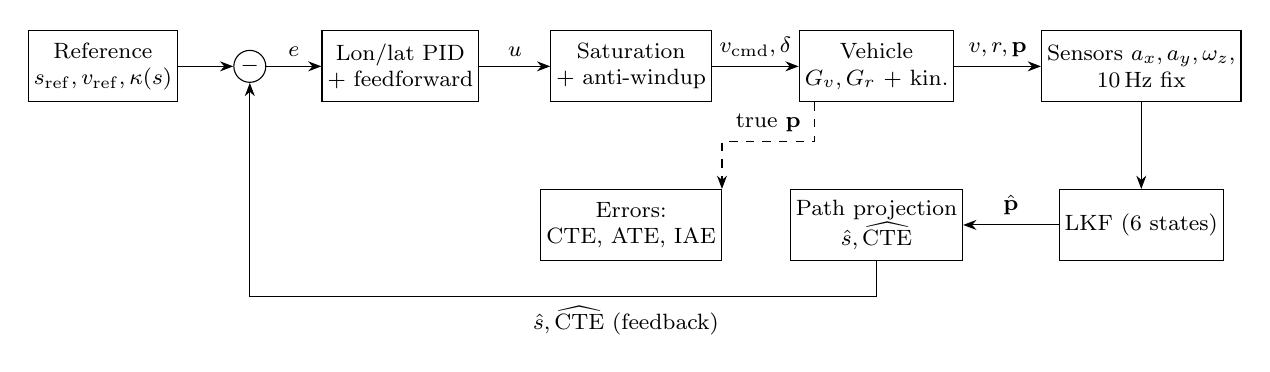
\begin{tikzpicture}[font=\footnotesize,>=Stealth,
  blk/.style={draw,rectangle,minimum height=0.9cm,minimum width=1.7cm,align=center,inner sep=2pt},
  sm/.style={draw,circle,inner sep=1pt}]
\node[blk] (ref) {Reference\\$s_\mathrm{ref},v_\mathrm{ref},\kappa(s)$};
\node[sm,right=0.7cm of ref] (sum) {$-$};
\node[blk,right=0.7cm of sum] (pid) {Lon/lat PID\\+ feedforward};
\node[blk,right=0.9cm of pid] (sat) {Saturation\\+ anti-windup};
\node[blk,right=1.1cm of sat] (veh) {Vehicle\\$G_v,G_r$ + kin.};
\node[blk,right=1.1cm of veh] (sen) {Sensors $a_x,a_y,\omega_z$,\\\SI{10}{Hz} fix};
\node[blk,below=1.1cm of sen] (lkf) {LKF (6 states)};
\node[blk,below=1.1cm of veh] (proj) {Path projection\\$\hat s,\widehat{\mathrm{CTE}}$};
\node[blk,below=1.1cm of sat] (err) {Errors:\\CTE, ATE, IAE};
\draw[->] (ref)--(sum);
\draw[->] (sum)--node[above]{$e$}(pid);
\draw[->] (pid)--node[above]{$u$}(sat);
\draw[->] (sat)--node[above]{$v_\mathrm{cmd},\delta$}(veh);
\draw[->] (veh)--node[above]{$v,r,\mathbf p$}(sen);
\draw[->] (sen)--(lkf);
\draw[->] (lkf)--node[above]{$\hat{\mathbf p}$}(proj);
\draw[->] (proj.south) -- ++(0,-0.45) -| node[pos=0.2,below]{$\hat s,\widehat{\mathrm{CTE}}$ (feedback)}(sum.south);
\draw[->,dashed] (veh.south west)++(0.2,0) -- ++(0,-0.5) -| node[pos=0.25,above]{true $\mathbf p$}(err.north east);
\end{tikzpicture}
\caption{Integrated closed loop. Estimated quantities feed the controllers; the \emph{true} position feeds the performance indices (dashed).}
\label{fig:block}
\end{figure*}

%=====================================================================
\section{System Identification and State-Space Model}\label{sec:id}
\textbf{ARX least squares.} Each channel is modelled as
\begin{equation}
y(k)=-\sum_{i=1}^{n_a}a_i\,y(k-i)+\sum_{j=1}^{n_b}b_j\,u(k-n_k-j+1)+e(k).
\label{eq:arx}
\end{equation}
With $\varphi(k)=[-y(k-1)\dots-y(k-n_a)\;u(k-n_k)\dots u(k-n_k-n_b+1)]$, stacked as $\Phi$ and $Y=[y(k)]$, the model $Y=\Phi\theta+e$, $\theta=[a_1..a_{n_a}\,b_1..b_{n_b}]^\top$, is linear in the parameters and the global least-squares optimum is
\begin{equation}
\hat\theta=(\Phi^\top\Phi)^{-1}\Phi^\top Y,
\label{eq:ls}
\end{equation}
computed by QR (\texttt{theta = Phi\textbackslash Y}); it agrees with the normal equations to $<10^{-12}$ ($\operatorname{cond}(\Phi^\top\Phi)\approx 5\!\times\!10^3$). The regression delay $n_k\ge1$ is imposed so that $G(z)$ is strictly proper and the loop has no algebraic loop.

\textbf{Inputs, outputs, protocol.} Longitudinal: $u=v_\mathrm{cmd}$, $y=v_\mathrm{wheel}$. Lateral: $y=r=\omega_z-b_g$ (gyro bias removed) and the static front end
\begin{equation}
u_\mathrm{lat}=\frac{v\tan\delta\,(1-c_s\delta^2)}{L\,(1+K_{us}v^2)},
\label{eq:ulat}
\end{equation}
a kinematic yaw-rate demand corrected for understeer ($K_{us}=\SI{\Kus}{s^2/m^2}$) and steering saturation ($c_s=\SI{\csat}{rad^{-2}}$; both fitted on identification data only). It makes $G_r$ speed-independent and LTI, and is exactly invertible to obtain $\delta$ from a demanded $u_\mathrm{lat}$ (gain scheduling idea of the lateral channel). Without it the validation fit is only \fitLatBase\,\% ; with speed correction only \fitLatSpeed\,\%.
The moving period ($v\ge\SI{1}{m/s}$, \SI{79}{s}) is cut into six contiguous blocks; blocks 1,3,5 identify, blocks 2,4,6 validate, so both sets cover the full speed range. Regressors never cross block borders and free-run simulations restart at each block start. The start-up dead zone and the slew-limited braking are excluded (strongly non-linear). Fit metrics: $\mathrm{NRMSE}=100(1-\|y-\hat y\|/\|y-\bar y\|)$ and $R^2$.

\textbf{Order selection.} $n_a,n_b\in\{1,2,3\}$, $n_k\in\{0,\dots,10\}$ (99 LS fits per channel), selected on the \emph{identification} free-run fit with a parsimony rule (fewest parameters within \SI{0.25}{points} of the best, then smallest $n_k\ge1$). The longitudinal channel is saturated at first order: extra parameters change the fit by $<0.15$ points while each extra sample of delay costs 1--2 points. The lateral channel needs a second-order denominator and $n_k=3$ (\SI{60}{ms}); the fit collapses for $n_k\ge6$.

\textbf{Identified transfer functions} ($T=\SI{\Tsamp}{s}$):
\begin{align}
G_v(z)&=\frac{\vBone\,z^{-1}}{1\vAone\,z^{-1}}=\frac{\vBone}{z-\vPoleV},\label{eq:Gv}\\
G_r(z)&=\frac{\latBone\,z^{-3}}{1\latAone\,z^{-1}+\latAtwo\,z^{-2}}.\label{eq:Gr}
\end{align}
$G_v$: $\tau_v=\SI{\vTauV}{s}$, DC gain \vGdc{} (unity tracking), one sample delay. $G_r$: poles $\latPoleRe\pm j\latPoleIm$, i.e.\ $\omega_n=\SI{\latWn}{rad/s}$, $\zeta=\latZeta$, delay \SI{60}{ms}, DC gain $k_\delta=\latKdelta$.

\textbf{Fits.} Table~\ref{tab:fit} and Fig.~\ref{fig:val} give the results. Both channels exceed the 90\,\% requirement on validation in free-run simulation (the honest metric; the one-step fit is optimistic). Caveat: a chronological hold-out (last 40\,\% of the run, almost constant speed) gives \fitLonChrono\,\% longitudinally (lateral \fitLatChrono\,\%) at the \emph{same} absolute RMSE (\SI{0.020}{m/s}); the NRMSE denominator is small there. \emph{Cross-check} with the System Identification Toolbox \texttt{arx} (MATLAB R2026a): the longitudinal parameters are identical ($\max|\Delta\theta|=\arxLon$); the lateral ones differ by at most \arxLat, because \texttt{arx} treats the initial samples of each segment differently. On the identical regression matrix our solution has the lower loss (MSE $7.99\times10^{-4}$ vs.\ $8.02\times10^{-4}$ for the \texttt{arx} parameters on segment 1), i.e.\ it is the exact minimiser of the stated problem~\eqref{eq:ls}.

\begin{table}[t]
\caption{Identification fits (NRMSE $\%$ / $R^2$), pooled over blocks}
\label{tab:fit}
\centering
\begin{tabular}{llcc}
\toprule
Channel & Set & One-step & Free-run \\
\midrule
Lon.\ $G_v$ & ident. & \fitLonIdOSA\,/\,\rLonIdOSA & \fitLonIdFree\,/\,\rLonIdFree \\
            & valid. & \fitLonVaOSA\,/\,\rLonVaOSA & \textbf{\fitLonVaFree}\,/\,\rLonVaFree \\
Lat.\ $G_r$ & ident. & \fitLatIdOSA\,/\,\rLatIdOSA & \fitLatIdFree\,/\,\rLatIdFree \\
            & valid. & \fitLatVaOSA\,/\,\rLatVaOSA & \textbf{\fitLatVaFree}\,/\,\rLatVaFree \\
\bottomrule
\end{tabular}
\end{table}

\begin{figure*}[t]
\centering
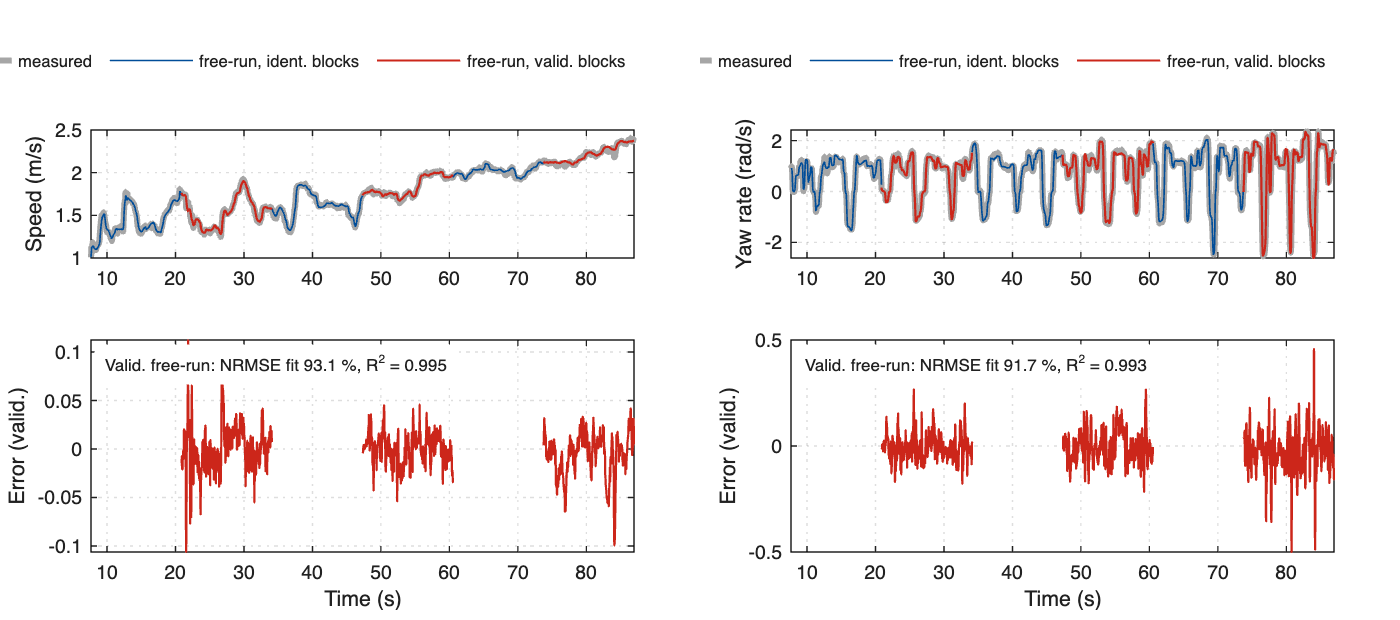
\includegraphics[width=0.6\textwidth]{figs/sysid_val.png}
\caption{Measured vs.\ free-run simulated output; red: validation blocks, blue: identification blocks. Left: longitudinal speed; right: yaw rate; lower panels: validation error.}
\label{fig:val}
\end{figure*}

\textbf{State-space model.} For $G(z)=B(\z)/A(\z)$ of order $n$ (delay samples included as states) the controllable canonical form is
\begin{equation}
A_c=\begin{bmatrix}0&I_{n-1}\\-a_n\;\cdots\;-a_1\end{bmatrix},\; B_c=e_n,\; C_c=[b_n\dots b_1],
\end{equation}
and the observable form is its dual ($A_o=A_c^\top$, $B_o=C_c^\top$, $C_o=B_c^\top$). Longitudinal ($n=1$): $A=\vPoleV$, $B=1$, $C=\vBone$. Lateral ($n=3$): last row of $A_c$ $=[0\;\;-\latAtwo\;\;\latAoneAbs]$, $C_c=[\latBone\;0\;0]$. \emph{Verification} (same $T$ for tf and ss): the maximum difference between transfer-function and state-space impulse, step and random-input responses over 400 samples is $<\tfssErr$ for both forms and both channels (also against the toolbox \texttt{step} of \texttt{tf}/\texttt{ss}); $\operatorname{rank}\mathcal C=\operatorname{rank}\mathcal O=n$ (1 and 3), so the realisations are controllable, observable and minimal in the sense that $A(\z)$ and $B(\z)$ share no root.

%=====================================================================
\section{Pole-Placement Discrete PID}\label{sec:pid}
\textbf{Controller.} Parallel form, backward-Euler integrator, filtered backward-difference derivative with pole $p_f=1/(1+NT)$:
\begin{align}
I(k)&=I(k-1)+K_iT\,e(k),\nonumber\\
D(k)&=p_fD(k-1)+\tfrac{K_d(1-p_f)}{T}\,\Delta e(k),\nonumber\\
u(k)&=K_pe(k)+I(k)+D(k),\; C(z)=\tfrac{N_c(z)}{(z-1)(z-p_f)},
\label{eq:pid}
\end{align}
with $N_c=c_2z^2+c_1z+c_0$, $c_2=K_p+K_iT+K_{df}$, $c_1=-[(1+p_f)K_p+p_fK_iT+2K_{df}]$, $c_0=p_fK_p+K_{df}$, $K_{df}=K_d(1-p_f)/T$.

\textbf{Plants.} Longitudinal loop (position $s$, input $v_\mathrm{cmd}$): $G_s(z)=G_v(z)\,T/(z-1)=bT/[(z-a)(z-1)]$ (order 2). Lateral loop (output cross-track error, input $u_\mathrm{lat}$), linearised at $v_0=\SI{2}{m/s}$: $G_{e}(z)=v_0T^2G_r(z)/(z-1)^2$ (order 5, 3-sample delay, type 2). Plant gain is positive in both, and the full-order models are used (no reduction).

\textbf{Closed-loop polynomial and desired poles.} With $G=N_p/D_p$ ($D_p$ monic of degree $n$, $N_p$ constant),
\begin{equation}
\Delta(z)=(z-1)(z-p_f)D_p(z)+N_c(z)N_p,\;\; \deg\Delta=n+2.
\label{eq:delta}
\end{equation}
The specification gives the dominant pair: $\omega_n=4/(\zeta t_{ss})$ ($2\,\%$ criterion), $s_{1,2}=-\zeta\omega_n\pm j\omega_n\sqrt{1-\zeta^2}$, $\mathrm{OS}=e^{-\pi\zeta/\sqrt{1-\zeta^2}}$ (4.6\,\% at $\zeta=0.7$), and $z_i=e^{s_iT}$. Two extra real poles $s_{3,4}=-\kappa\zeta\omega_n$ complete the set. We choose $\zeta=\lonZeta$, $t_{ss}^\mathrm{des}=\SI{\lonTssDes}{s}$, $\kappa=4$ (lon: $\omega_n=\SI{\lonWn}{rad/s}$) and $\zeta=\latZetaPID$, $t_{ss}^\mathrm{des}=\SI{\latTssDes}{s}$, $\kappa=2$ (lat: $\omega_n=\SI{\latWnPID}{rad/s}$), tighter than the required $t_{ss}\le\SI{2.5}{s}$ to leave margin for the non-ideal zeros.

\textbf{Coefficient matching (Diophantine equation).} Let $A_d(z)=\prod_{i=1}^4(z-z_i)$. For $n=2$ equating the four non-leading coefficients of~\eqref{eq:delta} with those of $A_d$ gives $p_f=\sum z_i-2-a$ and $c_2,c_1,c_0$ explicitly, then $K_p=[-c_1-p_fc_2-(2-p_f)c_0]/(1-p_f)^2$, $K_{df}=c_0-p_fK_p$, $K_iT=c_2-c_0-(1-p_f)K_p$. For the lateral plant ($n=5$, seven poles, four free parameters) the pair and the extra poles are placed exactly and the remaining three poles are the roots of an unknown monic residual $R(z)$:
\begin{equation}
(z-1)(z-p_f)D_p(z)+N_c(z)N_p=A_d(z)R(z).
\label{eq:dioph}
\end{equation}
Both sides are affine in $(p_f,c_2,c_1,c_0)$ and $R$, so matching gives a square $7\times7$ linear system. The residual poles come out fast ($|z|\le0.47$) and stable. Faster extra poles ($\kappa\ge3$) force $p_f>1$ (unrealisable), hence $\kappa=2$. A reduction of $G_r$ to its DC gain $k_\delta$ was rejected: it lowers the damping of the dominant pair from \latZetaPID{} to \latStaticZeta{} on the full model. Gains: Table~\ref{tab:gains}.

\begin{table}[t]
\caption{Pole-placement PID gains (lateral at $v_0=\SI{2}{m/s}$)}
\label{tab:gains}
\centering
\begin{tabular}{lcccc}
\toprule
Loop & $K_p$ & $K_i$ [1/s] & $K_d$ [s] & $p_f$ \\
\midrule
Lon.\ ($v_\mathrm{cmd}$ per m) & \lonKp & \lonKi & \lonKd & \lonPf \\
Lat.\ ($u_\mathrm{lat}$ per m) & \latKp & \latKi & \latKd & \latPf \\
\bottomrule
\end{tabular}
\end{table}

\textbf{Achieved poles and step metrics.} The roots of $\Delta(z)$ built by polynomial multiplication coincide with the desired poles to $10^{-6}$ (double-root sensitivity), also against \texttt{pole(feedback(CG,1))}. A PID adds two zeros (roots of $N_c$), giving 1-DOF overshoot of \lonOSoneDOF\,\% (lon) and \latOSoneDOF\,\% (lat) despite well-damped poles. Pole placement with zero cancellation fixes this with the prefilter $F(z)=N_c(1)z^2/N_c(z)$ (poles = PID zeros, all stable, unit DC gain), so $T_r(z)=N_c(1)N_pz^2/(A_d R)$ contains the placed poles only (closed form agrees with the simulated difference equations to $10^{-11}$). Table~\ref{tab:step} and Fig.~\ref{fig:steps} show that all specifications are met, also on the non-linear plant (lateral $0.5$\,m step: OS \nlLatOS\,\%, $t_{ss}$=\nlLatTss\,s).

\begin{table}[t]
\caption{Step metrics (full-order model, prefilter) vs.\ targets}
\label{tab:step}
\centering
\begin{tabular}{llccc}
\toprule
Loop & Metric & Target & Achieved & \\
\midrule
Lon. & $\zeta$ of dominant poles & $\ge0.7$ & \lonZeta & pass\\
     & 2\,\% settling time [s] & $\le2.5$ & \lonTss & pass\\
     & overshoot [\%] & $<10$ & \lonOS & pass\\
Lat. & $\zeta$ of dominant poles & $\ge0.7$ & \latZetaPID & pass\\
     & 2\,\% settling time [s] & $\le2.5$ & \latTss & pass\\
     & overshoot [\%] & $<10$ & \latOS & pass\\
\bottomrule
\end{tabular}
\end{table}

\begin{figure*}[t]
\centering
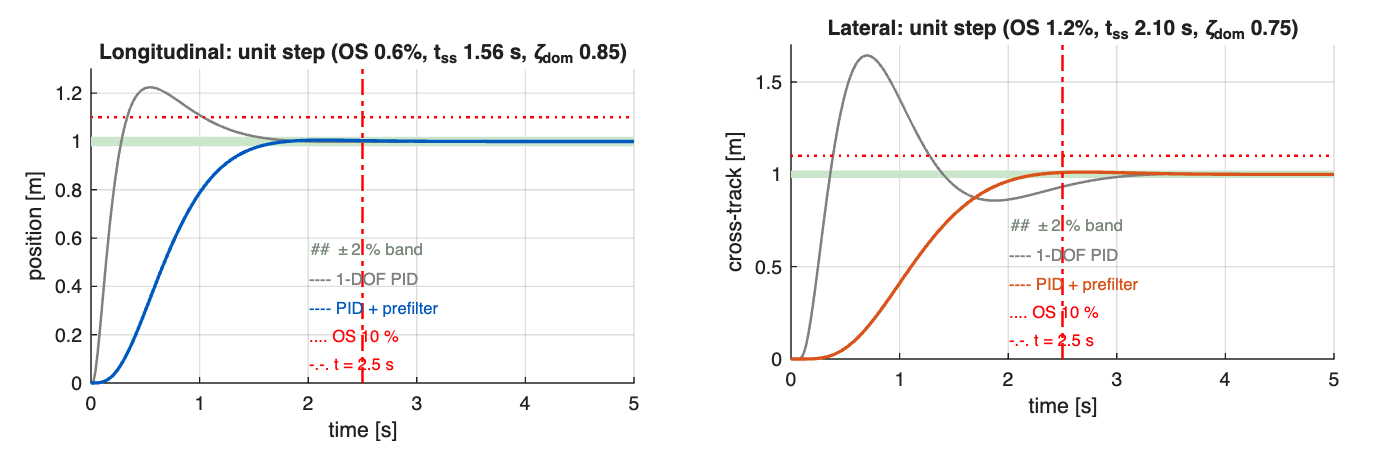
\includegraphics[width=0.6\textwidth]{figs/steps.png}\\[2pt]
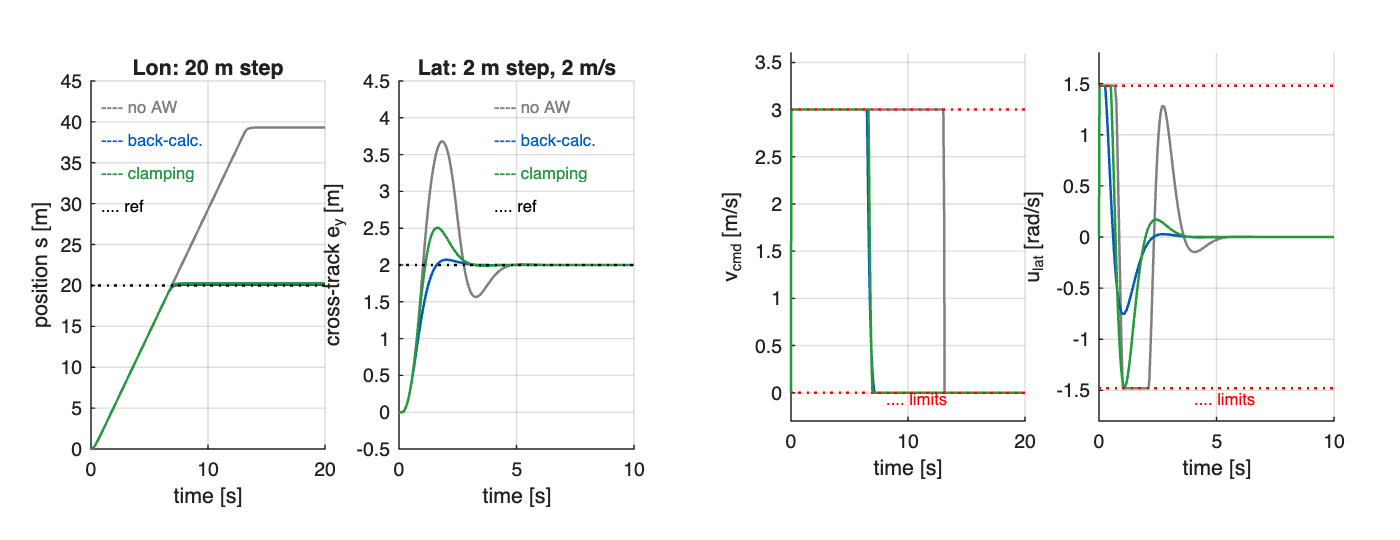
\includegraphics[width=0.72\textwidth]{figs/antiwindup.png}
\caption{Top: unit-step responses of the longitudinal (left) and lateral (right) loop, 1-DOF PID vs.\ PID with prefilter, $\pm2\,\%$ band, 10\,\% overshoot and \SI{2.5}{s} markers. Bottom: anti-windup with large steps (left pair: longitudinal \SI{20}{m} step, position and $v_\mathrm{cmd}$ with limits $[0,3]$\,m/s; right pair: lateral \SI{2}{m} step at \SI{2}{m/s}, $e_y$ and $u_\mathrm{lat}$ with limit $\pm1.48$\,rad/s). Panels in order: lon.\ position, lat.\ $e_y$, lon.\ $v_\mathrm{cmd}$, lat.\ $u_\mathrm{lat}$.}
\label{fig:steps}
\end{figure*}

\textbf{Saturation and anti-windup.} Limits are $0\le v_\mathrm{cmd}\le\SI{3}{m/s}$ and $|\delta|\le\SI{0.34}{rad}$, mapped through~\eqref{eq:ulat} to a speed-dependent $|u_\mathrm{lat}|\le\SI{1.48}{rad/s}$ at \SI{2}{m/s}. The feedforward is added before the limiter. With $u=\mathrm{sat}(u_\mathrm{un})$ the integrator uses back-calculation~\cite{astrom2006}
\begin{equation}
I(k)=I(k-1)+K_iT\,e(k)+T K_t(u-u_\mathrm{un}),\; K_t=\tfrac{1}{\sqrt{T_iT_d}},
\label{eq:aw}
\end{equation}
which is identical to the linear design when unsaturated. Fig.~\ref{fig:steps} (bottom): the longitudinal \SI{20}{m} step overshoots by \awLonNone\,\% without anti-windup (never settles; \awLonBC\,\% with back-calculation, \awLonCl\,\% clamping); the lateral \SI{2}{m} step by \awLatNone\,\% without, \awLatBC\,\% with back-calculation and \awLatCl\,\% with clamping. Because the lateral type-2 loop is only conditionally stable under saturation, anti-windup is mandatory.

\textbf{Gain scheduling.} The lateral plant gain is proportional to $v$ ($\dot e_y=v\psi_e$). Scaling $K_p,K_i,K_d$ by $v_0/v$ keeps the loop transfer function, hence all closed-loop poles, identical for any speed (characteristic polynomial difference $0$ at $v=1,2,3$\,m/s). Unscheduled, the damping at \SI{1}{m/s} falls to $\zeta=0.15$ ($t_{ss}=\SI{9.8}{s}$).

%=====================================================================
\section{Linear Kalman Filter}\label{sec:lkf}
\textbf{Model.} State $x=[p_X\;v_X\;p_Y\;v_Y\;b_x\;b_y]^\top$: map-frame position and velocity plus a residual accelerometer bias (random walk, body frame). The measured body accelerations are rotated by the heading $\psi$ \emph{outside} the filter ($\psi$ is a known exogenous signal from a complementary filter of bias-corrected gyro and the \SI{10}{Hz} heading fix), so the filter remains linear:
\begin{equation}
\begin{gathered}x_{k+1}=Fx_k+Gu_k+w_k,\quad z_k=Hx_k+\nu_k,\\ u=R(\psi)(a_\mathrm{meas}-b_\mathrm{cal}).\end{gathered}
\label{eq:kf}
\end{equation}
With $F_a=\begin{bsmallmatrix}1&T\\0&1\end{bsmallmatrix}$, $G_a=[T^2/2\;\;T]^\top$: $F=\begin{bsmallmatrix}\mathrm{blkdiag}(F_a,F_a)&-G_0R(\psi_k)\\0&I_2\end{bsmallmatrix}$, $G=[G_0;0]$ with $G_0=\mathrm{blkdiag}(G_a,G_a)$, $H=\begin{bsmallmatrix}1&0&0&0&0&0\\0&0&1&0&0&0\end{bsmallmatrix}$. The prediction runs at \SI{50}{Hz}; the update (Joseph form) only when a \SI{10}{Hz} position fix arrives.

\textbf{Noise statistics and $Q$, $R$.} From the \SI{23.8}{s} of standstill in the real log: $\sigma_{a_x}=\SI{\sigAxStand}{m/s^2}$, $\sigma_{a_y}=\SI{\sigAyStand}{m/s^2}$, gyro $\SI{\sigGyro}{rad/s}$. In motion (high-pass residual) the accelerometer noise is about ten times larger because of vibration: $\sigma_{a_x}=\SI{\sigAxMot}{m/s^2}$, $\sigma_{a_y}=\SI{\sigAyMot}{m/s^2}$. The input noise is mapped through $G$ (white-noise-acceleration model; isotropic $\sigma_w=\sqrt{(\sigma_{a_x}^2+\sigma_{a_y}^2)/2}$ so that $Q$ stays constant while the body noise rotates):
\begin{equation}
Q=\mathrm{blkdiag}\!\big(\sigma_w^2G_aG_a^\top,\;\sigma_w^2G_aG_a^\top,\;q_bT\,I_2\big),\;\; R=\sigma_z^2I_2.
\label{eq:qr}
\end{equation}
$\sigma_w=\SI{\sigWStand}{m/s^2}$ (standstill, used in simulation) or \SI{\sigWMot}{m/s^2} (in motion, real run). The bias random-walk intensity $q_b=\qbRW\,(\si{m/s^2})^2/\si{s}$ comes from the change of the two standstill means $93$\,s apart. $R$ is the variance of the position fix: the fix is emulated at \SI{10}{Hz} (GNSS/LiDAR-localisation-like, \SI{0.5}{m} at full scale) with $\sigma_z=\SI{\sigZ}{m}$ per axis (heading fix $\SI{\sigPsi}{rad}$); the log's own particle-filter jitter (\SI{4}{mm}) is only a lower bound of the real error and is therefore not used. Because the estimate depends only on $Q/R$, Fig.~\ref{fig:sens} scales both: in simulation the justified values are optimal (best RMSE at $Q$ scale \simBestQ, \simRMSEcm\,cm; NIS \simNIS, expected 2).

\textbf{Consistency.} The normalised innovation squared has expectation 2 (two measurements)~\cite{barshalom2001}. In simulation mean NIS is \simNIS{} (95\,\% band \simNISband), innovations are white, mean position NEES \simNEES{} (expected 2): the filter is consistent. On the real run it is not: mean NIS \realNIS{} with the in-motion $Q$, and \realNISstand{} with the standstill $Q$ (over-confident; RMSE \realRMSEstandQ\,m). The reason is that in motion the IMU does not agree with the accelerations implied by the particle-filter pose (lateral correlation $\approx$\realCorrAy, longitudinal $\approx$\realCorrAx; roll/pitch gravity leakage and vibration), so the accelerometer error is coloured, not white. Raising $Q$ by $\times\realBestQ$ would lower the real-run RMSE to \realBestRMSE\,cm (nominal \realRMSEcm\,cm), but we keep the measured value rather than tune to the result.

\begin{figure}[t]
\centering
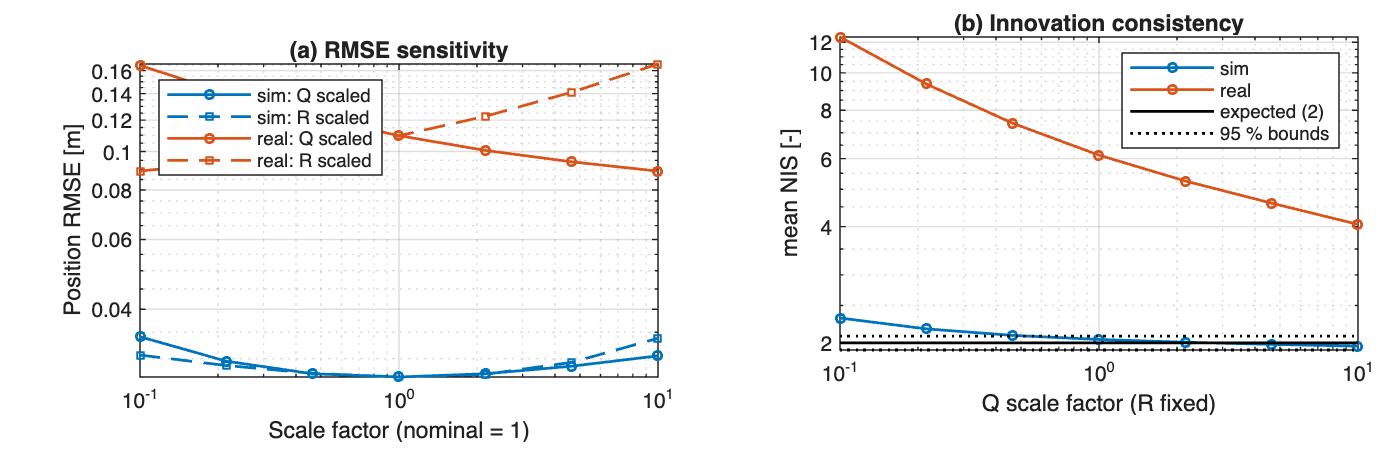
\includegraphics[width=\columnwidth]{figs/lkf_sens.png}
\caption{Sensitivity of the LKF to $Q$ and $R$ scaled around the design values (nominal $=1$). Left: position RMSE; right: mean NIS vs.\ $Q$ scale (expected value 2).}
\label{fig:sens}
\end{figure}

\textbf{Accuracy.} RMSE is $\sqrt{\mathrm{mean}(e_X^2+e_Y^2)}$ over the whole record against the noise-free reference (simulated truth, or the particle-filter pose on the real run); the baseline is double integration of the same rotated accelerometers from the true initial state, and the ``raw fixes'' are the zero-order-held noisy \SI{10}{Hz} positions. Table~\ref{tab:lkf} shows the results. The reduction versus raw double integration is $\ge$\realRedInt\,\% in both cases (requirement 70\,\%), (integration alone drifts by hundreds of metres). Against the position \emph{measurement} the result must be read with care: in simulation the LKF reduces the RMSE by \simRedHeld\,\% vs.\ held fixes (\simRedFixAt\,\% vs.\ fixes at their instants), but on the real run it is only on par with held fixes (\realRedHeld\,\%) and worse at the fix instants (\realRedFixAt\,\%) because of the coloured in-motion accelerometer error above. An optional wheel-speed velocity update ($v_\mathrm{wheel}[\cos\hat\psi,\sin\hat\psi]^\top$, $\sigma_v=\SI{0.05}{m/s}$) lowers the simulated RMSE from \simRMSEcm\,cm to \simWheelRMSE\,m, but on the real run it is \emph{worse} (\realWheelRMSE\,m): it assumes no side slip, which fails when the car slides in corners. It is therefore not part of the real-data filter of Table~\ref{tab:lkf}; Sec.~\ref{sec:nav} uses it in simulation only.

\begin{table}[t]
\caption{Position RMSE [m] and LKF reduction [\%]}
\label{tab:lkf}
\centering
\begin{tabular}{lcc}
\toprule
 & Simulation & Real run \\
\midrule
Raw double integration & \simRawInt & \realRawInt \\
Raw, bias-corrected & \simRawBC & \realRawBC \\
Raw fixes (held, \SI{50}{Hz}) & \simFixHeld & \realFixHeld \\
LKF, 4 states (no bias) & \simLKFfour & \realLKFfour \\
\textbf{LKF, 6 states} & \textbf{\simLKF} & \textbf{\realLKF} \\
\midrule
Reduction vs.\ raw integration & \simRedInt\,\% & \realRedInt\,\% \\
Reduction vs.\ held fixes & \simRedHeld\,\% & \realRedHeld\,\% \\
\bottomrule
\end{tabular}
\end{table}



%=====================================================================
\section{Closed-Loop Navigation on the Scaled Circuit}\label{sec:nav}
\textbf{Track scaling.} The Mexico City centreline and widths of the TUMFTM database~\cite{heilmeier2020} are scaled by $1{:}10$ (an F1 car of \SI{5.5}{m} vs.\ our \SI{0.54}{m}), smoothed by a periodic spline and re-parametrised by arc length: $L=\SI{\trackLen}{m}$ (\SI{\trackLenFS}{m} full scale), width \SIrange{\trackWmin}{\trackWmax}{m}, maximum curvature \SI{\kappaMax}{m^{-1}} (radius \SI{\rMin}{m}). The rubric limits are scaled identically: $\mathrm{CTE}_{\max}\le\SI{0.15}{m}$ and $\mathrm{RMSE}_\mathrm{CTE}\le\SI{0.05}{m}$ correspond to \SI{1.5}{m}/\SI{0.5}{m} at full scale.

\textbf{Speed profile and reference.} $v_\mathrm{ref}(s)=\min\big(v_\mathrm{max},\sqrt{a_\mathrm{lat}/|\kappa|}\big)$ with $v_\mathrm{max}=\SI{\vTrackMax}{m/s}$, $a_\mathrm{lat}=\SI{\aLat}{m/s^2}$, additionally limited by what the steering can realise ($|\kappa|\le0.8\,k_\delta\,u_\mathrm{lat}(v,\delta_{\max})/v$) and by cyclic forward/backward acceleration limits ($+1.5$/$-2.0$\,m/s$^2$). The time-parametrised reference $s_\mathrm{ref}(t)$ gives a lap time of \SI{\lapTime}{s} (mean \SI{\vMean}{m/s}).

\textbf{Simulation plant and sensors.} The identified $G_v$, $G_r$ (as difference equations, with delays) and eq.~\eqref{eq:ulat} drive a kinematic model ($\dot\psi=r$, $\dot x=v\cos\psi$, $\dot y=v\sin\psi$) with the saturations of Sec.~\ref{sec:pid}. Sensors: $a_x=\Delta v/T$, $a_y=vr$, gyro $r$, with the \emph{in-motion} noise levels and bias of Sec.~\ref{sec:lkf}, a wheel-speed measurement ($\sigma=\SI{0.0072}{m/s}$, in-motion level from the log), a \SI{10}{Hz} position/heading fix, and the LKF $Q$ built on exactly the same noise level. The plant additionally has the steering-servo rate limit from the servo specification, \SI{0.15}{s} per \SI{60}{\degree}, i.e.\ $(\pi/3)/0.15=\SI{6.98}{rad/s}$, applied to the commanded angle (the controller is unaware of it; the plant has no servo dead zone). The LKF in the loop fuses the wheel-speed measurement at the fix instants (the optional 03-design of Sec.~\ref{sec:lkf}, $H$ with four rows); \textbf{this assumes no side slip} and, as shown there, was worse on the real data, so the nominal result is a simulation result. The first \SI{5}{s} are a standstill for bias calibration (not in the lap time). The estimated position is projected onto the track (windowed nearest-vertex search with foot-point refinement) to produce $\hat s$ and signed $\widehat{\mathrm{CTE}}$; \emph{all metrics use the true position}.

\textbf{Control.} Longitudinal: $e_s=s_\mathrm{ref}-\hat s$, feedforward $u_{ff}=(v_\mathrm{ref}(k{+}1)-a\,v_\mathrm{ref}(k))/b$ (plant inverse of $G_v$), saturation, back-calculation. Lateral: scheduled gains, curvature feedforward $u_{ff}=\hat v\,\kappa(\hat s+\hat vt_{la})/k_\delta$ with look-ahead $t_{la}=\SI{\tLA}{s}$ (delay plus part of the servo lag), $\delta=\mathrm{lat\_inverse}(u_\mathrm{lat},\hat v)$. Above \SI{1}{m/s} the derivative term is applied to the measurement only, $u_D=-K_d(v_0/\hat v)\,\dot{\widehat{e}}_y$, with $\dot{\widehat e}_y=\hat{\mathbf v}\cdot\mathbf n(\psi_\mathrm{path})$ from the LKF velocity (no kick at the \SI{10}{Hz} fix jumps); the designed differenced D is kept below \SI{1}{m/s} (start-up). $K_p,K_i,K_d,p_f$ are unchanged.

\textbf{Metrics.} $\mathrm{IAE}=\int|\mathrm{CTE}|\,dt$; $\mathrm{ATE}=s(t)-s_\mathrm{ref}(t)$; position RMSE against the time-parametrised reference; track margin $=$ distance to the nearest boundary minus half the car width (\SI{0.15}{m}).

\begin{figure*}[t]
\centering
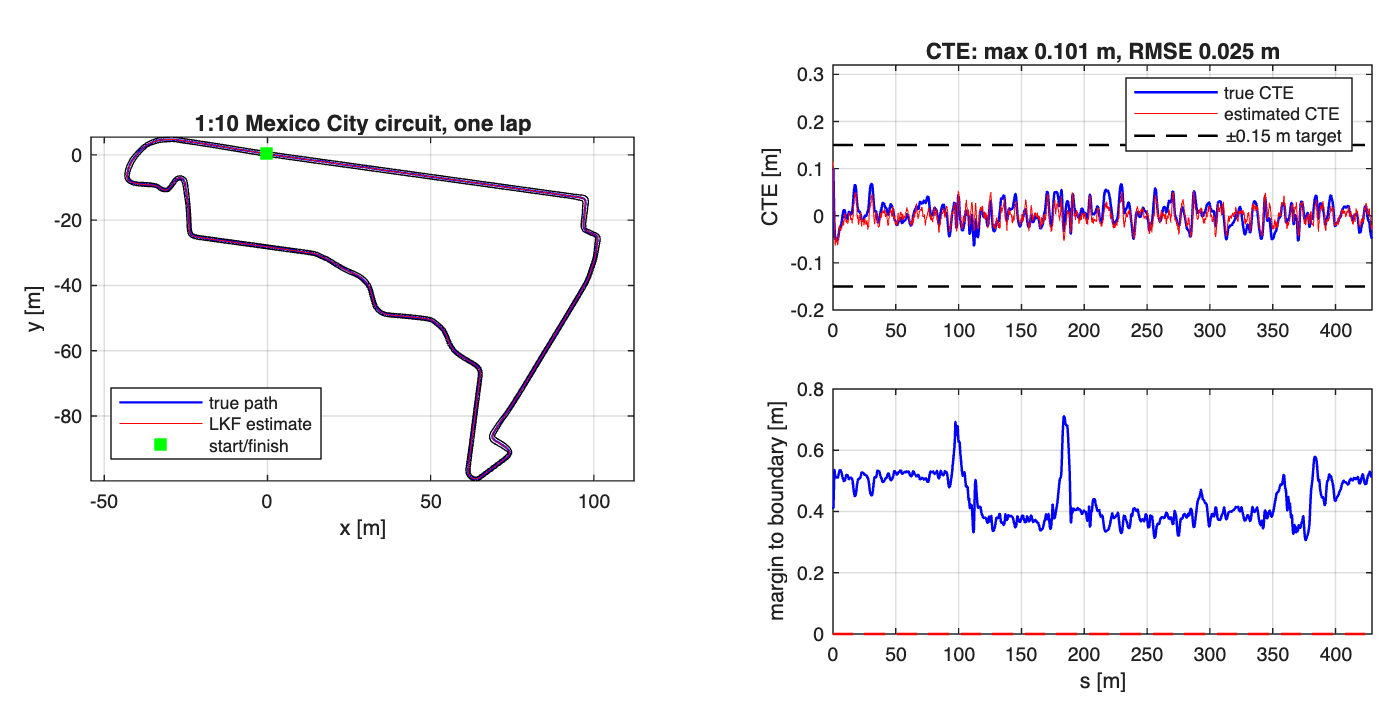
\includegraphics[width=0.62\textwidth]{figs/nav.png}
\caption{Nominal lap (LKF feedback). Left: scaled Mexico City circuit, true path (black) and LKF estimate (red). Right: true and estimated CTE versus arc length with the $\pm\SI{0.15}{m}$ limit (top), and margin to the boundary (bottom).}
\label{fig:nav}
\end{figure*}

\textbf{Results.} Fig.~\ref{fig:nav} and Table~\ref{tab:nav} give the nominal run (seed 1). The car completes the full \SI{\trackLen}{m} lap in \SI{\lapTime}{s} and never leaves the track (minimum margin \SI{\margin}{m}). $\mathrm{CTE}_{\max}=\SI{\CTEmax}{m}$ and $\mathrm{RMSE}_{\mathrm{CTE}}=\SI{\CTErmse}{m}$ meet the scaled limits, equivalent to \SI{\CTEmaxFS}{m}/\SI{\CTErmseFS}{m} at full scale. The maximum is the initial \SI{0.1}{m} start offset; after the first \SI{3}{s} it is \SI{\CTEafter}{m}. Four indices are reported (CTE, IAE, ATE, position RMSE), more than the two required. The LKF position error during the lap is \SI{\navLKFpos}{m} RMS against \SI{\navRaw}{m} for raw double integration (reduction \navRed\,\%; \navRedFix\,\% versus the raw \SI{\navFixRMSE}{m} fixes).

\begin{table}[t]
\caption{Nominal lap metrics (1:10) vs.\ targets}
\label{tab:nav}
\centering
\resizebox{\columnwidth}{!}{%
\begin{tabular}{lccccc}
\toprule
Metric & Target & LKF fb. & Ideal fb. & $\times10$ & \\
\midrule
$\mathrm{CTE}_{\max}$ [m] & $\le0.15$ & \CTEmax & \idealCTEmax & \CTEmaxFS & pass\\
$\mathrm{RMSE}_\mathrm{CTE}$ [m] & $\le0.05$ & \CTErmse & \idealCTErmse & \CTErmseFS & pass\\
IAE [m\,s] & -- & \CTEiae & \idealIAE & -- & \\
ATE RMSE / max [m] & -- & \ATErmse\,/\,\ATEmax & \idealATE\,/\,\idealATEmax & -- & \\
Position RMSE [m] & -- & \posRMSEnav & \idealPosRMSE & -- & \\
Lap time [s] & -- & \lapTime & \lapTime & -- & \\
Track margin [m] & $>0$ & \margin & \idealMargin & -- & pass\\
\bottomrule
\end{tabular}}
\end{table}

\textbf{LKF vs.\ ideal feedback, and what mattered.} With true-state feedback $\mathrm{RMSE}_\mathrm{CTE}$ is \idealCTErmse\,m (the maximum is again the start offset), so the loop remains \emph{estimation-limited}: the LKF feedback costs a factor $\approx2$. An ablation over ten seeds shows what reduced it. With the accelerometer+fix LKF (\navNoFusedLKF\,m position RMSE) and the differenced D term the worst-seed $\mathrm{CTE}_{\max}$ was \ablActe\,m and the steering rate RMS \steerRateOld\,rad/s (violent chatter). Moving the D term to the LKF velocity alone made it \emph{worse} (worst \ablCcte\,m) because the velocity error times the long derivative time $T_d=K_d/K_p=\SI{0.5}{s}$ acts like a 3--4\,cm offset. Fusing the wheel speed halved the LKF error (\navFusedLKF\,m), and only then did the measurement-based D help, lowering the steering rate RMS to \steerRateNew\,rad/s at unchanged CTE. The gain thus comes from estimate quality and rests on the no-side-slip assumption (steering RMS \deltaRMS\,rad, commanded rate RMS \deltaRateRMS\,rad/s vs.\ \idealDeltaRate{} ideal).

\textbf{Robustness.} Table~\ref{tab:rob} varies the noise seed (ten seeds), the speed limit and the plant gains $\pm15\,\%$ with unchanged controllers. All runs pass: over ten seeds $\mathrm{CTE}_{\max}$ lies in \seedCTElo--\seedCTEhi\,m and $\mathrm{RMSE}_\mathrm{CTE}$ in \seedRMSElo--\seedRMSEhi\,m, with margin $\ge$\,\marginMinRob\,m. The worst plant-mismatch case is a lateral gain $\times0.85$ ($\mathrm{CTE}_{\max}=\SI{\GrWorstCTE}{m}$, still $<\SI{0.15}{m}$ but with little margin; $\mathrm{RMSE}_\mathrm{CTE}=\SI{0.034}{m}$). At $v_\mathrm{max}=\SI{3}{m/s}$ the speed command saturates during acceleration and ATE grows to \SI{\ATEvThree}{m} RMS, yet the CTE targets hold; \SI{2}{m/s} costs \lapIncrease\,\% more lap time.

\begin{table}[t]
\caption{Sensitivity and robustness runs (LKF feedback). CTE and RMSE in m, IAE in m\,s, lap in s; ``worst'' = largest value (smallest margin) over ten seeds.}
\label{tab:rob}
\centering
\setlength{\tabcolsep}{3pt}
\footnotesize
\resizebox{\columnwidth}{!}{%
\begin{tabular}{lccccccc}
\toprule
Run & Lap & $\mathrm{CTE}_{\max}$ & $\mathrm{RMSE}_\mathrm{CTE}$ & IAE & ATE$_\mathrm{rms}$ & margin & $\le$ limits\\
\midrule
Nominal (seed 1) & \RobNominal \\
Ideal state fb. & \RobIdeal \\
Standstill-level noise & \RobStand \\
Seeds 1--10, worst & \RobSeeds \\
$v_\mathrm{max}=2.0$\,m/s & \RobVtwo \\
$v_\mathrm{max}=3.0$\,m/s & \RobVthree \\
$G_r$ gain $\times0.85$ & \RobGrLo \\
$G_r$ gain $\times1.15$ & \RobGrHi \\
$G_v$ gain $\times0.85$ & \RobGvLo \\
$G_v$ gain $\times1.15$ & \RobGvHi \\
\bottomrule
\end{tabular}}
\end{table}

\textbf{Simulink implementation.} The complete loop of Fig.~\ref{fig:block} is also built as a Simulink model (\texttt{nav\_closed\_loop.slx}, fixed-step discrete solver, $T_s=\SI{0.02}{s}$; Fig.~\ref{fig:slx}). Each block is a MATLAB Function block calling the \emph{same} \texttt{pid\_step}, \texttt{lkf\_step} and projection functions as the script, with internal states as persistent variables and a Unit Delay on the plant state to break the algebraic loop. Driven with the same noise sequence, it reproduces the script: maximum difference in true position \SI{\simulinkPos}{m}, in LKF estimate \SI{\simulinkEst}{m}, in steering \SI{\simulinkDelta}{rad}, and identical CTE ($\mathrm{CTE}_{\max}=\SI{0.1015}{m}$, $\mathrm{RMSE}=\SI{0.0249}{m}$), i.e.\ rounding level.

\begin{figure*}[t]
\centering
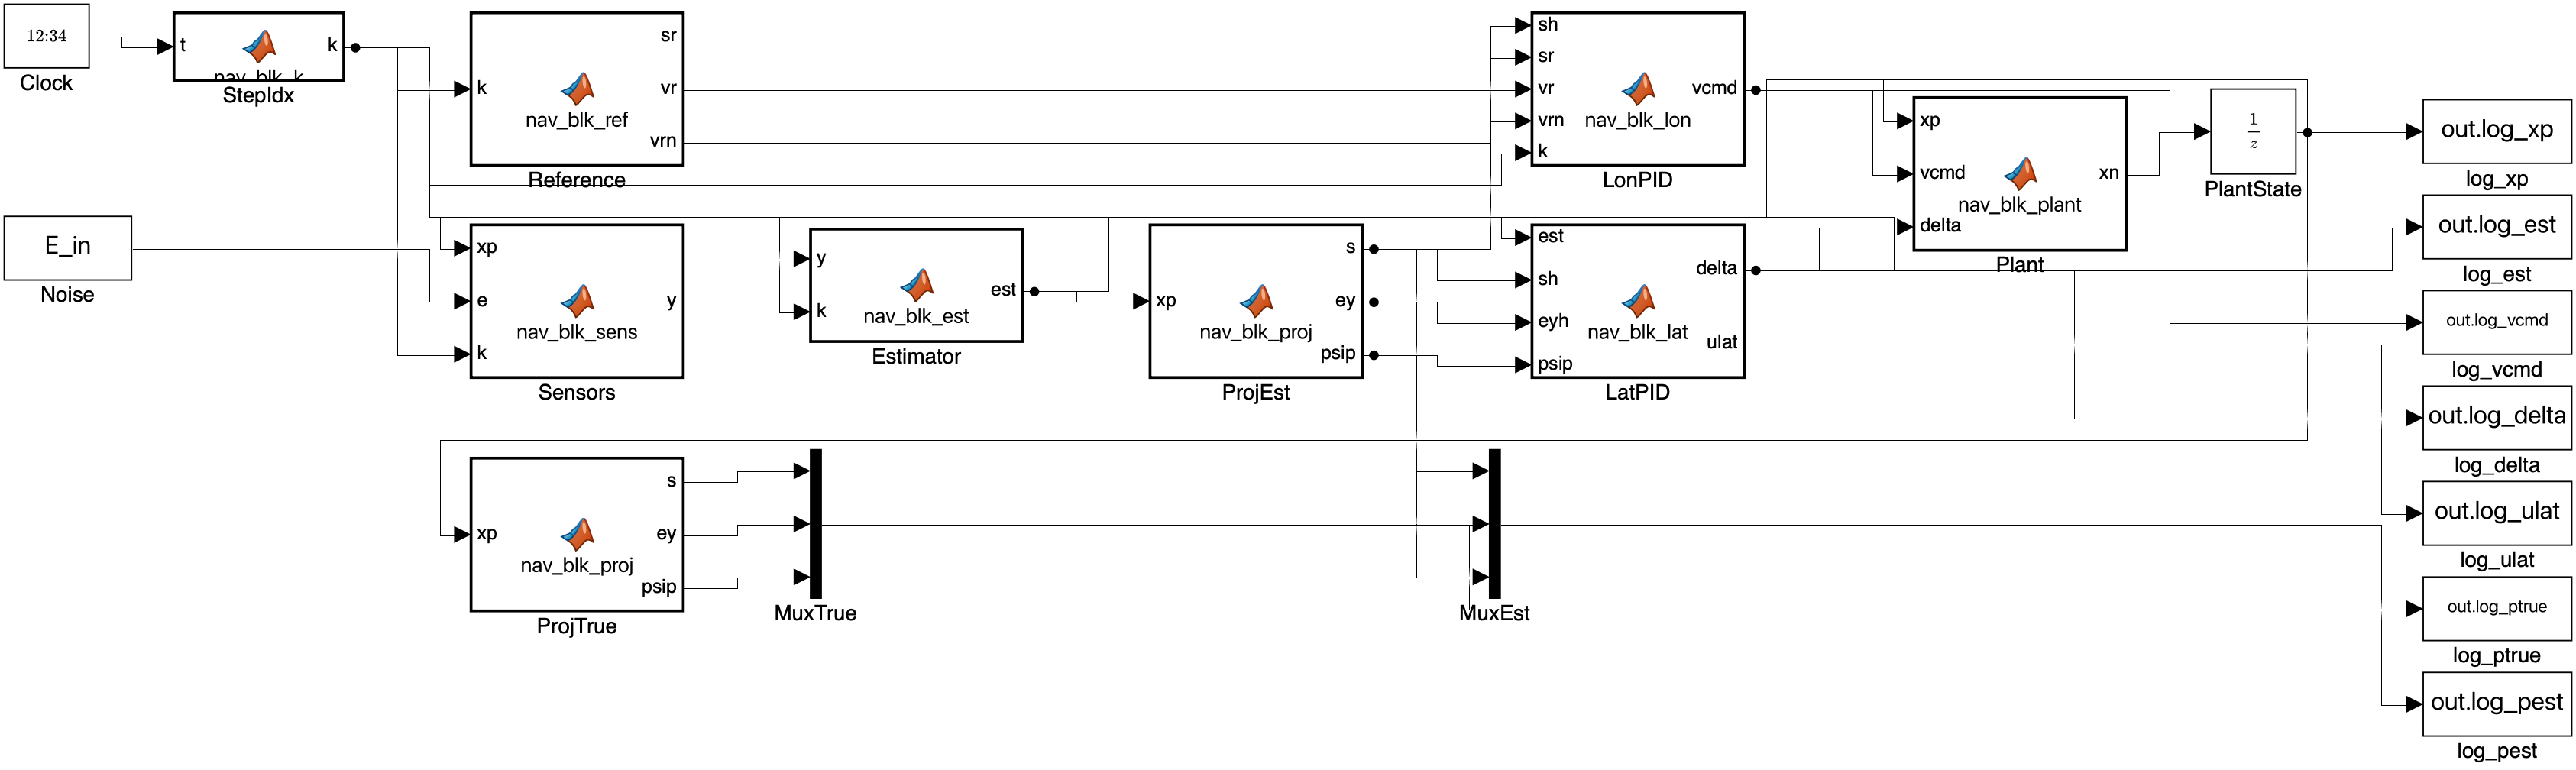
\includegraphics[width=0.62\textwidth]{figs/simulink.png}
\caption{Simulink model of the integrated closed loop: reference, sensors with noise input, estimator (calibration, heading filter, LKF), path projection, longitudinal and lateral PID, plant with Unit Delay, and logging.}
\label{fig:slx}
\end{figure*}

\textbf{Compliance with the targets.} Table~\ref{tab:comp} collects every criterion.
\begin{table}[t]
\caption{Requirements and achieved values}
\label{tab:comp}
\centering
\footnotesize
\setlength{\tabcolsep}{3pt}
\resizebox{\columnwidth}{!}{%
\begin{tabular}{llccl}
\toprule
Requirement & Target & Achieved & Status & Sec. \\
\midrule
Fit, lon./lat., valid. free-run [\%] & $\ge90$ & \fitLonVaFree\,/\,\fitLatVaFree & pass & III\\
$R^2$ valid. lon./lat. & report & \rLonVaFree\,/\,\rLatVaFree & pass & III\\
tf $\leftrightarrow$ ss equivalence & exact & $<\tfssErr$ & pass & III\\
Damping $\zeta$ lon./lat. & $\ge0.7$ & \lonZeta\,/\,\latZetaPID & pass & IV\\
Settling time $t_{ss}$ [s] & $\le2.5$ & \lonTss\,/\,\latTss & pass & IV\\
Overshoot [\%] & $<10$ & \lonOS\,/\,\latOS & pass & IV\\
Saturation: OS with anti-windup [\%] & bounded & \awLonBC\,/\,\awLatBC & pass & IV\\
RMSE reduction vs.\ raw integr. [\%] & $\ge70$ & \simRedInt\,/\,\realRedInt & pass & V\\
$Q$, $R$ from sensor statistics & justified & stats., NIS & pass & V\\
$\mathrm{CTE}_{\max}$ [m] (1:10 / $\times10$) & $\le0.15$ / $1.5$ & \CTEmax\ / \CTEmaxFS & pass & VI\\
$\mathrm{RMSE}_\mathrm{CTE}$ [m] (1:10 / $\times10$) & $\le0.05$ / $0.5$ & \CTErmse\ / \CTErmseFS & pass & VI\\
Full lap, inside track [m margin] & $>0$ & \margin & pass & VI\\
Indices (CTE, ATE, IAE, RMSE) & $\ge2$ & 4 & pass & VI\\
Paper length [pages] & $\le8$ & \pages & pass & --\\
\bottomrule
\end{tabular}}
\end{table}

%=====================================================================
\section{Conclusions and Learning Reflection}\label{sec:conc}
\textbf{What worked.} A linear least-squares ARX model with one explicit solver was enough: a first-order longitudinal and a second-order-plus-delay lateral model explain real validation data to \fitLonVaFree\,\% and \fitLatVaFree\,\%, and every added parameter beyond that was demonstrably useless. Placing poles on the \emph{full} model through the Diophantine system, instead of on a reduced model, was decisive: the DC-gain reduction looked fine analytically but collapsed the damping from \latZetaPID{} to \latStaticZeta{}. The prefilter turned a \latOSoneDOF\,\% overshoot into \latOS\,\% without touching the loop, and back-calculation made large steps safe where the lateral type-2 loop would otherwise circle. The LKF reduced position error by more than 99.9\,\% against double integration, and its $Q$/$R$ from measured statistics sit at the optimum of the sensitivity sweep in simulation. Finally, the 1:10 scaling lets the rubric limits be checked on a realistic circuit: \SI{\CTEmaxFS}{m}/\SI{\CTErmseFS}{m} equivalent full-scale CTE, robust over ten noise seeds and $\pm15\,\%$ gain errors, and the Simulink implementation reproduces the script to rounding level.

\textbf{Limitations.} (i) The model is identified from a single open-loop run; validation uses alternating blocks of the same run, not a second experiment, and the longitudinal chronological hold-out gives only \fitLonChrono\,\% because of the small output variance (identical absolute error). The start-up dead zone and slew-limited braking are outside the linear model. (ii) The lateral channel is a Hammerstein-type model: the static nonlinearity~\eqref{eq:ulat} (understeer, steering saturation) carries about 6 points of fit and is valid only for $v\ge\SI{1}{m/s}$. (iii) The PID zeros give large 1-DOF overshoot; the prefilter solves reference steps but is not used for the moving reference, where feedforward plays that role, and the derivative filter pole is restricted by the lateral dynamics ($\kappa\le2$). (iv) Closed-loop accuracy is estimation-limited: $\mathrm{RMSE}_\mathrm{CTE}$ is \CTErmse\,m with LKF vs.\ \idealCTErmse\,m with true state. Our best result depends on fusing the wheel speed in the LKF, which assumes no side slip and was \emph{worse} on the real log (\realWheelRMSE\,m vs.\ \realRMSEcm\,cm), so the nominal CTE is a simulation result; without it the worst-seed $\mathrm{CTE}_{\max}$ exceeded the limit (\ablActe\,m). (v) The real accelerometer noise in motion is coloured, so on real data the LKF is consistent only in simulation (NIS \realNIS{} vs.\ 2) and is merely on par with raw fixes; the 70\,\% requirement is met against raw integration but not against the real measured position. (vi) The lap is simulated on the identified linear model without tyre slip, servo dead zone or fix latency; the servo is modelled by its rate limit (\SI{6.98}{rad/s}) without dead zone, and the \SI{10}{Hz} position fix is emulated (noise \SI{\sigZ}{m}), so the result bounds, but does not replace, an on-track test.

\textbf{What we learned.} Quoting the fit of a model is meaningless without the protocol: one-step fits are all above 96\,\% while free-run, block-restarted validation gives 92--93\,\%, and the chronological hold-out reveals the dependence on excitation. Noise must be measured in the operating regime: standstill statistics are ten times optimistic and led to an over-confident filter (NIS \realNISstand). Reporting seed variance exposed that our first design failed the CTE limit in one of ten seeds; the cure was better estimation, not more control tuning (a velocity-based D term alone made it worse).

\textbf{Future work.} (1) A second identification experiment (closed-loop or different speed profile) for true cross-validation, with a Box--Jenkins/instrumental-variable structure for coloured noise. (2) Measure the servo rate limit and dead zone on the real car, and replace the no-side-slip wheel-speed update by a slip-aware velocity measurement model. (3) Run the design on the real vehicle with the LiDAR particle-filter fix instead of the emulated one.

\footnotesize\bibliographystyle{IEEEtran}
\bibliography{refs}
\end{document}
